\title{Tímaflækjur}
\author{Bergur Snorrason}
\date{\today}

\begin{document}

\frame{\titlepage}

\env{frame}
{
	\frametitle{Tímaflækjur}
	\env{itemize}
	{
		\item<1-> Látum $f, g \colon [0, \infty) \mapsto \mathbb{R}$.
		\item<2-> Við segjum að fall $g$ sé í menginu $\mathcal{O}(f)$ ef til eru rauntölur $c > 0$ og $x_0 > 0$ þannig að
		\[
			|g(x)| \leq c \cdot |f(x)|
		\]
		fyrir öll $x > x_0$.
		\item<3-> Þetta þýðir í raun að fallið $|g|$ verður á endanum minna en $c \cdot |f|$.
		\item<4-> Þessi lýsing undirstrikar að $f$ er efra mat á $g$, það er að segja $g$ hagar sér ekki verr en $f$.
		\item<5-> Ef $g \in \mathcal{O}(f)$ og $f \in \mathcal{O}(g)$ þá segjum við að $f \in \Theta(g)$ (og $g \in \Theta(f)$).
	}
}

\env{frame}
{
	\frametitle{Dæmi}
	\env{itemize}
	{
		\item<1-> Tökum nokkur dæmi.
		\item<2-> Ef $f \in \mathcal{O}(g)$ og $r > 0$ þá er $r \cdot f \in \mathcal{O}(g)$.
		\item<3-> Ef $f_1 \in \mathcal{O}(g_1)$ og $f_2 \in \mathcal{O}(g_2)$ þá er $f_1 \cdot f_2 \in \mathcal{O}(g_1 \cdot g_2)$.
		\item<4-> Dæmin fyrir ofan gilda ef ,,$\mathcal{O}$'' er skipt út fyrir ,,$\Theta$''.
		\item<5-> Ef $p$ er $n$-ta stigs margliða þá er $p \in \Theta(x^n)$.
		\item<6-> Ef $p$ er $n$-ta stigs margliða og $q$ er $m$-ta stigs margliða með $n < m$ þá er $p \in \mathcal{O}(q)$,
					en $q \not \in \mathcal{O}(p)$.
		\item<7-> Við höfum að $\log x \in \mathcal{O}(x)$ en $x \not \in \mathcal{O}(\log x)$.
		\item<8-> Nú er $\log x^n = n \cdot \log x$, svo ef $p$ er $n$-ta stigs margliða þá er $\log p \in \mathcal{O}(\log x)$.
	}
}

\env{frame}
{
	\frametitle{Í forritun}
	\env{itemize}
	{
		\item<1-> Takið eftir að í stað þessa að segja ,,$f \in \mathcal{O}(g)$'' er oft sagt ,,$f = \mathcal{O}(g)$'' eða ,,$f$ er $\mathcal{O}(g)$''.
		\item<2-> Ef forrit framkvæmir $T(n)$ aðgerðir, með $T \in \mathcal{O}(f)$,
					segjum við að \emph{tímaflækja} (e. \emph{time complexity}) forritsins sé $\mathcal{O}(f)$.
		\item<3-> Skoðum nú nokkur forrit og ákvörðum tímaflækjur þeirra.
	}
}

\env{frame}
{
	\code{code/daemi1.c}
	\env{itemize}
	{
		\item<2-> Hér er ekkert inntak svo forritið hefur tímaflækjuna $\mathcal{O}($\onslide<all:2->{$\,1\,$}$)$.
	}
}

\env{frame}
{
	\code{code/daemi2.c}
	\env{itemize}
	{
		\item<2-> Forritið les inn töluna $n$ og reiknar svo summuna $1 + 2 + \dots + n$.
		\item<3-> Þetta er gert með forlykkju sem keyrir $n$ sinnum.
		\item<4-> Hvert skipti eru tvær tölur lagðar saman.
		\item<5-> Svo þetta forrit er $\mathcal{O}($\onslide<6- | handout:2->{$\,n\,$}$)$.
	}
}

\env{frame}
{
	\code{code/daemi3.c}
	\env{itemize}
	{
		\item<2-> Forritið les inn töluna $n$ og reiknar svo summu.
		\item<3-> Summan er reiknuð með tvöfaldri forlykkju.
		\item<4-> Ytri forlykkjan keyrir $n$ sinnum og seinni keyrir aldrei oftar en $n/2$ sinnum.
		\item<5-> Svo tímaflækja forritsins er $\mathcal{O}($\onslide<6- | handout:2->{$n^2$}$)$.
	}
}

\env{frame}
{
	\code{code/daemi4.c}
	\env{itemize}
	{
		\item<2-> Sjáum fyrst að lykkjan í \ilcode{main(...)} keyrir $n - 1$ sinnum.
		\item<3-> Hún kallar síðan á fallið \ilcode{len(...)}.
		\item<4-> Það fall hefur eina \ilcode{while}-lykkju sem deilir tölunni $n$ með $k$, án afgangs, þar til $n$ er orðin núll.
		\item<5-> Þetta fallið \ilcode{len(...)} hefur því tímaflækjuna $\mathcal{O}($\onslide<6- | handout:2->{$\log n$}$)$.
		\item<7-> Í heildina hefur forritið því tímaflækjuna $\mathcal{O}($\onslide<8- | handout:3->{$n \log n$}$)$.
	}
}

\env{frame}
{
	\code{code/daemi5.c}
	\env{itemize}
	{
		\item<2-> Hér erum við með endurkvæmt fall.
		\item<3-> Við sjáum að ef $n \geq 2$ þá kallar \ilcode{fib(n)} tvisvar á sjálft sig.
		\item<4-> Svo þetta forrit er $\mathcal{O}($\onslide<5- | handout:2->{$2^n$}$)$.
		\item<6-> Það er hægt að fá betra mat (við getum minnkað veldisstofninn).
	}
}

\env{frame}
{
	\env{itemize}
	{
		\item<1-> Skoðum skiladæmið \emph{Reiknirit}.
		\item<2-> Fyrsta lína inntaksins inniheldur heiltölu $n$.
		\item<3-> Síðan koma $n$ heiltölur $a_1, a_2, \dots, a_n$.
		\item<4-> Gerum ráð fyrir að við séum með forrit sem gerir eftirfarandi:
		\env{itemize}
		{
			\item<5-> Prentar tölurnar.
			\item<6-> Fjarlægir öll eintök af algengustu tölunni í listan.
			\item<7-> Endurtekur skrefin að ofan þar til listinn er tómur.
		}
		\item<8-> Dæmið snýst um að finna hversu margar tölur eru prentaðar í heildina.
		\item<9-> Tökum dæmi.
	}
}

\env{frame}
{
	\env{itemize}
	{
		\item<1-> Gerum ráð fyrir að tölurnar í inntakinu séu $1, 2, 1, 4, 4$.
		\item<2-> Þá myndi forritið í dæminu prenta:
		\item<3->[] \code{code/reiknirit.out}
		\item<4-> Svo það prentar $9$ tölur.
	}
}

\env{frame}
{
	\env{itemize}
	{
		\item<1-> Ein leið til að leysa þetta dæmi er að útfæra forritið.
		\item<2-> Við þurfum þá að geta fjarlægt algengasta stakið.
	}
}

\env{frame}
{
	\selectcode{code/reiknirit.c}{3}{37}
}

\env{frame}
{
	\env{itemize}
	{
		\item<1-> Þetta forrit leysir dæmið (að því sem ég best veit).
		\item<2-> Nú er spurning hvort það sé nógu hratt.
		\item<3-> Í dæminu á Kattis er gefið að $n \leq 10^6$.
		\item<4-> Reynum nú að ákvarða tímaflækjuna.
		\item<5-> Sjáum aftur útfærsluna.
	}
}

\env{frame}
{
	\selectcode{code/reiknirit.c}{11}{37}
}

\env{frame}
{
	\env{itemize}
	{
		\item<1-> Í fyrsta lagi röðum við listanum, sem er $\mathcal{O}($\onslide<2->{$n \log n$}$)$.
		\item<3-> Síðan erum við með \ilcode{while}-lykkju, sem gerir ekkert annað en að kalla á fallið \ilcode{fjarlaegja\_algengasta\_stakid(...)}.
		\item<4-> Í versta falli fjarlægjum við eitt stak í einu, svo þessi \ilcode{while}-lykkja keyrir allt að $n$ sinnum.
		\item<5-> Í fallinu \ilcode{fjarlaegja\_algengasta\_stakid(...)} eru tvær lykkjur, hvor um sig keyrir $n$ sinnum.
		\item<6-> Takið eftir að $n$ er þá lengd listans á þeim tímapunkti.
		\item<7-> Fallið \ilcode{fjarlaegja\_algengasta\_stakid(...)} hefur því tímaflækjuna $\mathcal{O}($\onslide<8->{$\,n\,$}$)$.
		\item<9-> Forritið í heild sinni hefur því tímaflækjuna $\mathcal{O}($\onslide<10->{$n^2$}$)$.
	}
}

\env{frame}
{
	\env{itemize}
	{
		\item<1-> Rifjum upp að $n \leq 10^6$ og tímaflækjan er $\mathcal{O}(n^2)$.
		\item<2-> Er þetta nógu hratt til að fá \ilcode{AC}?
		\item<3-> Nú segir \emph{$10^8$ relgan} okkur að tímamörk dæmisins þurfi að vera $(10^6)^2 \cdot 10^{-8} = 10^4$ sekúndur.
		\item<4-> Svo er ekki og þessi lausn er því að fara að fá \ilcode{TLE}.
		\item<5->[] 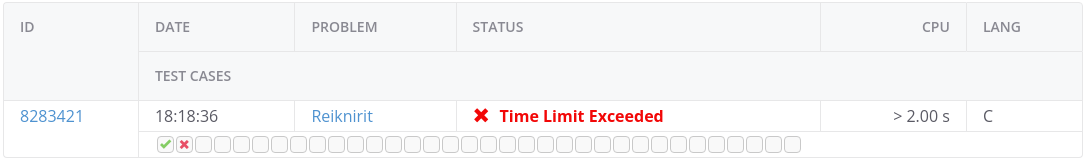
\includegraphics[scale = 0.25]{fig/tle}
	}
}

\env{frame}
{
}

\end{document}
